\section{Модель прямоугольного Изинга}

В данном разделе мы будем рассматривать зависимость наблюдаемых модели Изинга от формы решетки: в частности, от отношения сторон в прямоугольной решётке

\subsection{Расчёт критических кумулянтов для модели прямоугольного Изинга}

Кумулянт Биндера для модели Изинга в критической точке расчитывается по формуле:
\begin{equation}
\label{eq:Cumulant}
U_{4} = 1 - \frac{\la m^{4} \ra}{3 * (m^{2})^{2}}
\end{equation}

где $\la m^{2} \ra$ - средний квадрат удельной намагниченности, $\la m^{4} \ra$ - средная удельная намагниченность в четвертой степени. 

Для сравнения значения кумулянтов модели прямоугольного Изинга с разными размерами, но одинаковым отношением сторон (так же Aspect Ratio или r), так, что число спинов составляет L * rL были проведены симуляции модели на основе алгоритма из проектной работы Сорокина Никиты \cite{Schro} и Камиллы Файзулиной \cite{SAW} - для этого были взяты длины 50, 100, 200 и 400 и отношения сторон 1/4, 1/2, 3/4 при $2 * 10^{6}$ итераций.

\begin{figure}[!h]
    \centering
    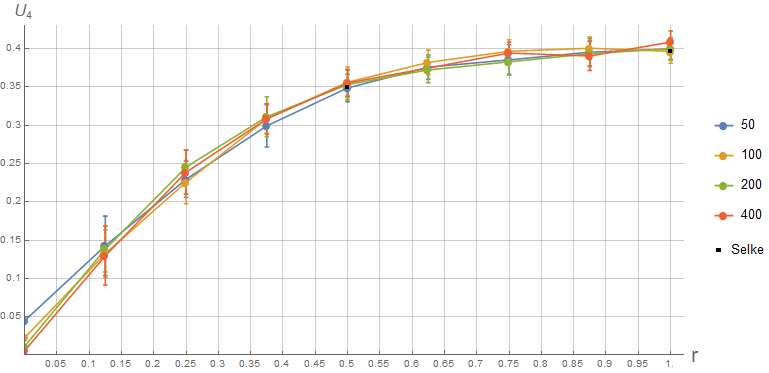
\includegraphics[width=100mm]{Sections/Images/CumulantOBC.png}
    \caption{График зависимости значения кумулянта Биндера в крит. точке от Aspect Ratio при открытых гран. условиях}
    \label{fig:CumulOBC}
\end{figure}

\begin{figure}[!h]
    \centering
    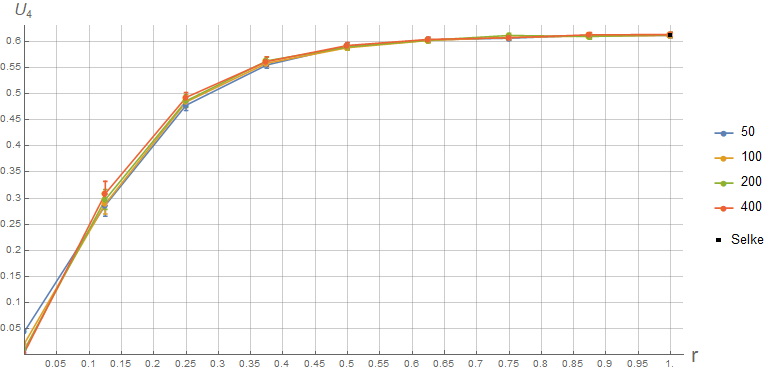
\includegraphics[width=100mm]{Sections/Images/CumulantPBC.png}
    \caption{График зависимости значения кумулянта Биндера в крит. точке от Aspect Ratio при периодических гран. условиях}
    \label{fig:CumulPBC}
\end{figure}

Крайние левые точки в отметке нуля являются расчётами для модели одномерного Изинга (где длина цепочки равна соответствующей стороне в двумерном изинге). Так, в случае открытых гран. условий (рис. \ref{fig:CumulOBC}) и периодических (рис. \ref{fig:CumulPBC}) значения кумулянта стремится к нулю с увеличением длины цепочки(см. Проект6.pdf\cite{Git}).
Черными точками отмечены значения критического кумулянта из работы Уолтера Сельке - 0.396 ± 0.002 для квадратной модели и 0.349 ± 0.002 для прямоугольной с отношением сторон r = 1/2 при открытых гран. условий. Для периодического случая квадратной модели критический кумулянт равен 0.61069\cite{Selke}.

Эти же значения отмечены в графиках \ref{fig:CumulOBCL} и \ref{fig:CumulPBCL} зависимости крит. кумулянта от обратной длины стороны как крайние левые (в нуле - так обозначен случай термодинамического предела).

\begin{figure}[!h]
    \centering
    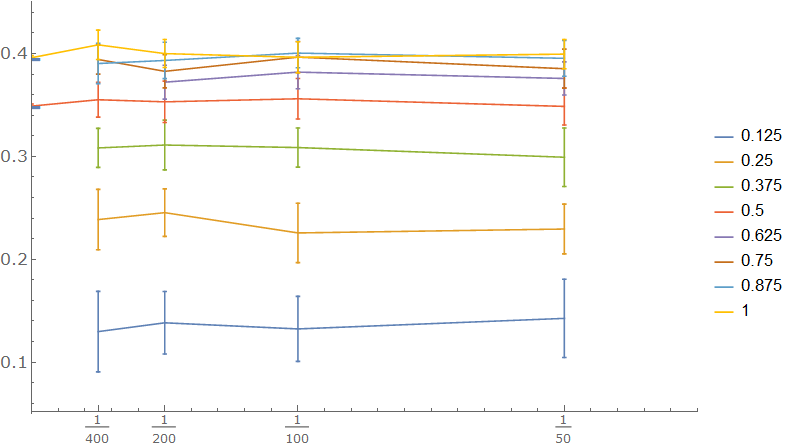
\includegraphics[width=100mm]{Sections/Images/CumulantOBCL.png}
    \caption{График зависимости значения кумулянта Биндера в крит. точке от обратной длины стороны при открытых гран. условиях}
    \label{fig:CumulOBCL}
\end{figure}

\begin{figure}[!h]
    \centering
    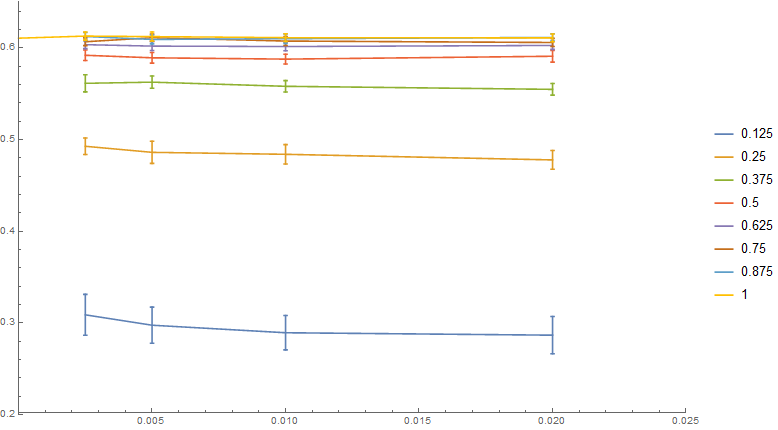
\includegraphics[width=100mm]{Sections/Images/CumulantPBCL.png}
    \caption{График зависимости значения кумулянта Биндера в крит. точке от обратной длины стороны при периодических гран. условиях}
    \label{fig:CumulPBCL}
\end{figure}

Учитывая погрешность в расчётах симуляций, зависимость от обратной длины прямоугольника 1/L не наблюдается.

\subsection{Сравнение модели Изинга и модели взаимодействующих непересекающихся блужданий}

Здесь мы рассмотрим основные понятия в модели взаимодействующих блужданий (Self-Avoiding Walks, SAWs), связанные с их формой и сравним их с прямоугольной моделью в тех же условиях. 

Важнейшим параметром в описании полученной симуляциями Монте-Карло блуждания является радиус инерции, численно равный среднему квадратическому расстоянию частиц от положения среднего арифметического центра модели (сумма $w_{k}$ в скобке):

\begin{equation}\label{eq:Rg}
    R^{2}_{g} = \frac{1}{N+1} \sum^{N}_{i=0}\left(w_{i} - \frac{1}{N+1}\sum^{N}_{k=0}w_{k}\right)^2 = \frac{1}{2(N+1)^{2}}\sum^{N}_{i,j=0}(w_{i} - w_{j})^{2}
\end{equation}

Так же для описания модели применяется тензор инерции - матрица, $\alpha\beta-$й элемент которой расчитывается по формуле:

\begin{equation}\label{eq:Ten_G1}
    Q_{N,\alpha\beta} = \frac{1}{2(N+1)^{2}} \sum^{N}_{i,j=0}(w_{i,\alpha} - w_{j, \alpha})(w_{i,\beta} - w_{j, \beta})
\end{equation}

Так же можно представить более простую формулу для  $\alpha\beta-$го элемента матрицы, численно идентичную \eqref{eq:Ten_G1}, но использующую другой метод вычислений:

\begin{equation}\label{eq:Ten_G2}
    Q_{N,\alpha\beta} = \frac{1}{(N+1)} \sum_{i=0}^{N} w_{i, \alpha} w_{i, \beta}
\end{equation}

Из последнеё формулы очевидно, что i-й диагональный элемент тензора инерции численно равны квадрату среднего квадратического значения i-й координаты по всем частицам модели.

Так как полученная матрица симметричная, то существует такой поворот, преобразующий её в диагональную (т.е., приводящий систему в Жорданов базис с собственными значениями по диагонали, и нулевыми недиагональными элементами), причём так, чтобы значения на диагонали были положительными и упорядоченными по невозрастанию.

В нашем двумерном случае, 

\begin{equation*}
    Q_{N} = \left(
    \begin{array}{cc}
      q_{1} & 0 \\
      0 & q_{2}
    \end{array} \right),\ 0 < q_{2} \leq q_{1}
\end{equation*}

Отметим так же, что сумма диагональных элементов тензора инерции равна квадрату радиуса инерции и инвариантна. Тогда определим ещё один показатель формы:

\begin{align*}
    s_{1} &= \frac{\la q_{1} \ra_{N}}{\la R_{g}^{2} \ra_{N}}\\
    s_{2} &= 1 - s1 = \frac{\la q_{2} \ra_{N}}{\la R_{g}^{2} \ra_{N}}\\
    r12 &= \frac{s1}{1-s1}
\end{align*}

Учитывая, что в $s_{1}$ и $s_{2}$ значения в числителе и знаменателе являются квадратами средних квадратичных значений, то следует вывод, что $\sqrt{r_{12}}$ является знакомым нам отношением сторон из предыдущего подраздела, только в данном случае это отношение не сторон прямоугольника, а полуосей эллипса инерции, который образует полученая симуляциями модель-блуждание.

Пример работы симуляции и расчётов формы эллипса инерции можно увидеть в Проект9.pdf\cite{Git}